% Copyright (c)  2019  FSC.
% Permission is granted to copy, distribute and/or modify this document
% under the terms of the GNU Free Documentation License, Version 1.3
% or any later version published by the Free Software Foundation;
% with no Invariant Sections, no Front-Cover Texts, and no Back-Cover Texts.
% A copy of the license is included in the section entitled "GNU
% Free Documentation License".

\begin{figure}[H]
	\centering
	\caption{Gabbia logica della pagina di login.}
	\label{fig:gabbie-logiche:login}
	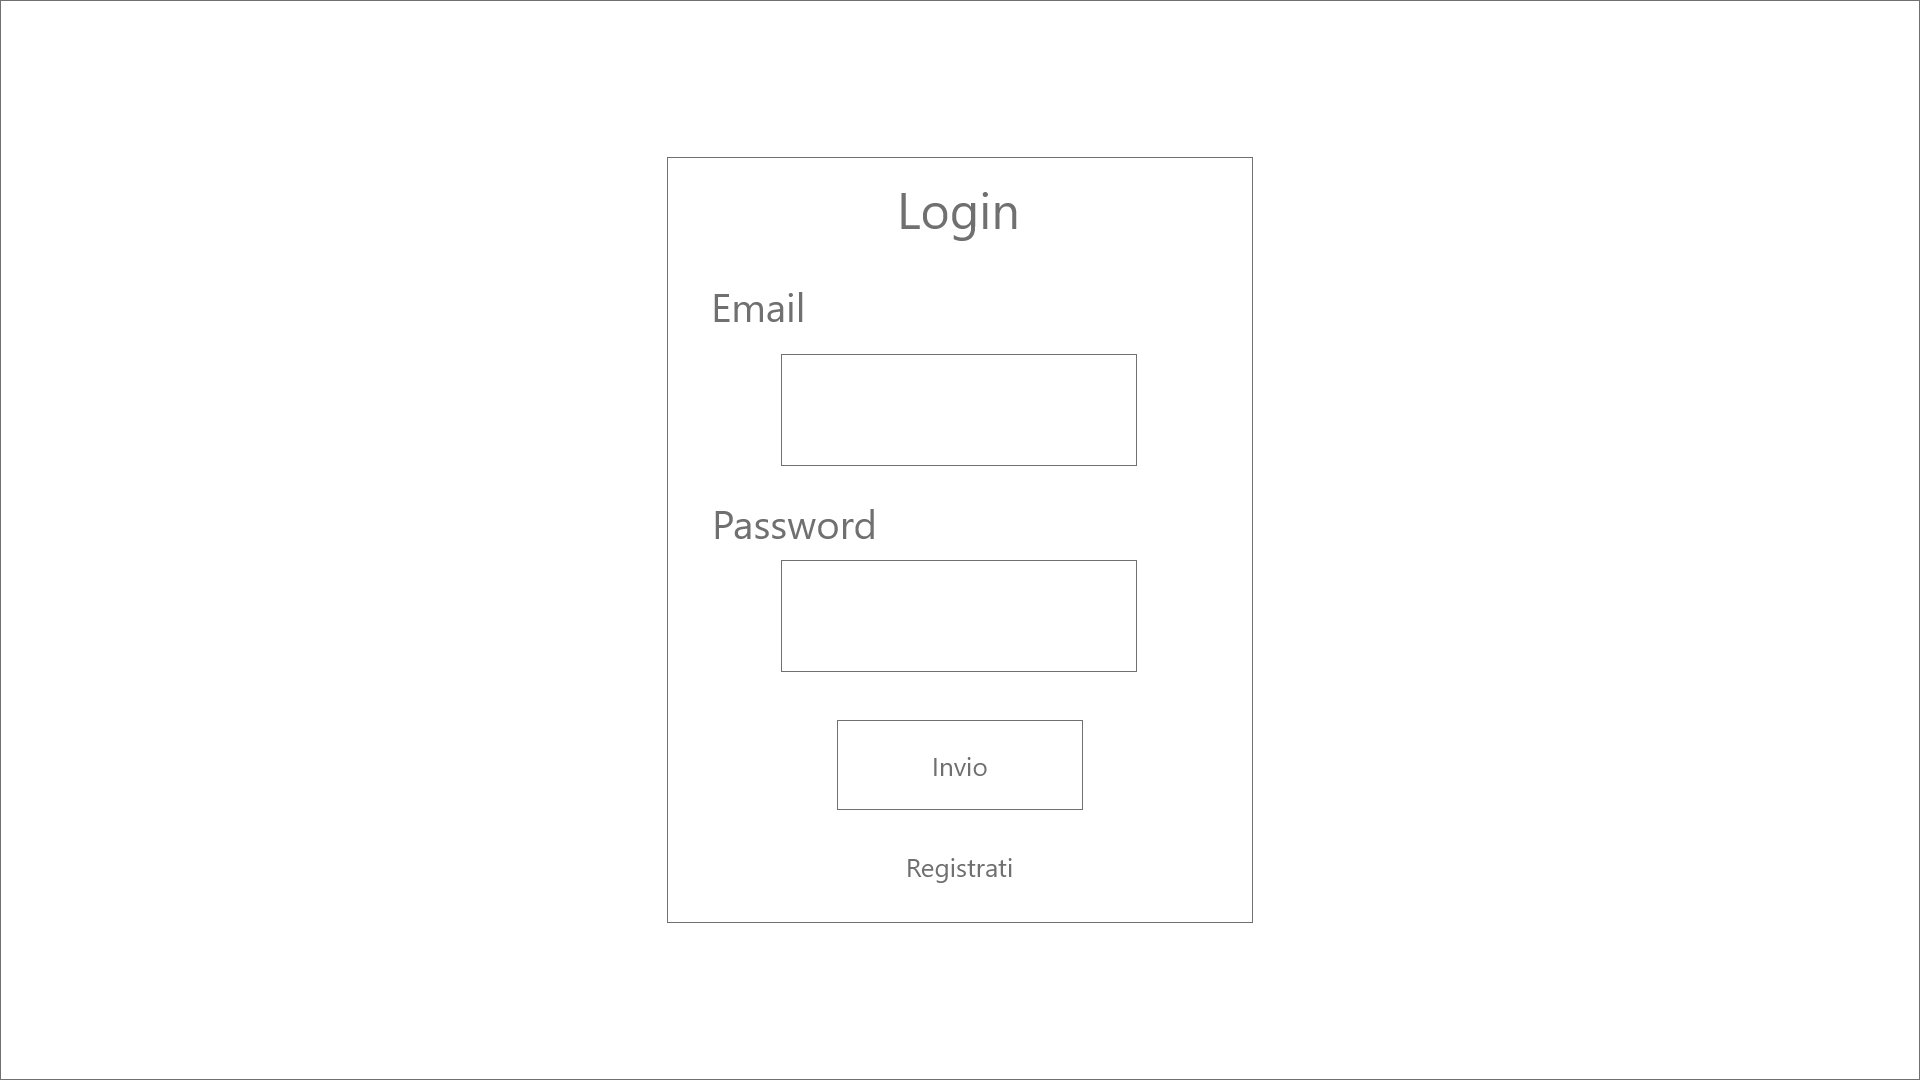
\includegraphics[width=\textwidth]{images/gabbie-logiche/Login}
\end{figure}

\begin{figure}[H]
	\centering
	\caption{Gabbia logica della landing page.}
	\label{fig:gabbie-logiche:landing-page}
	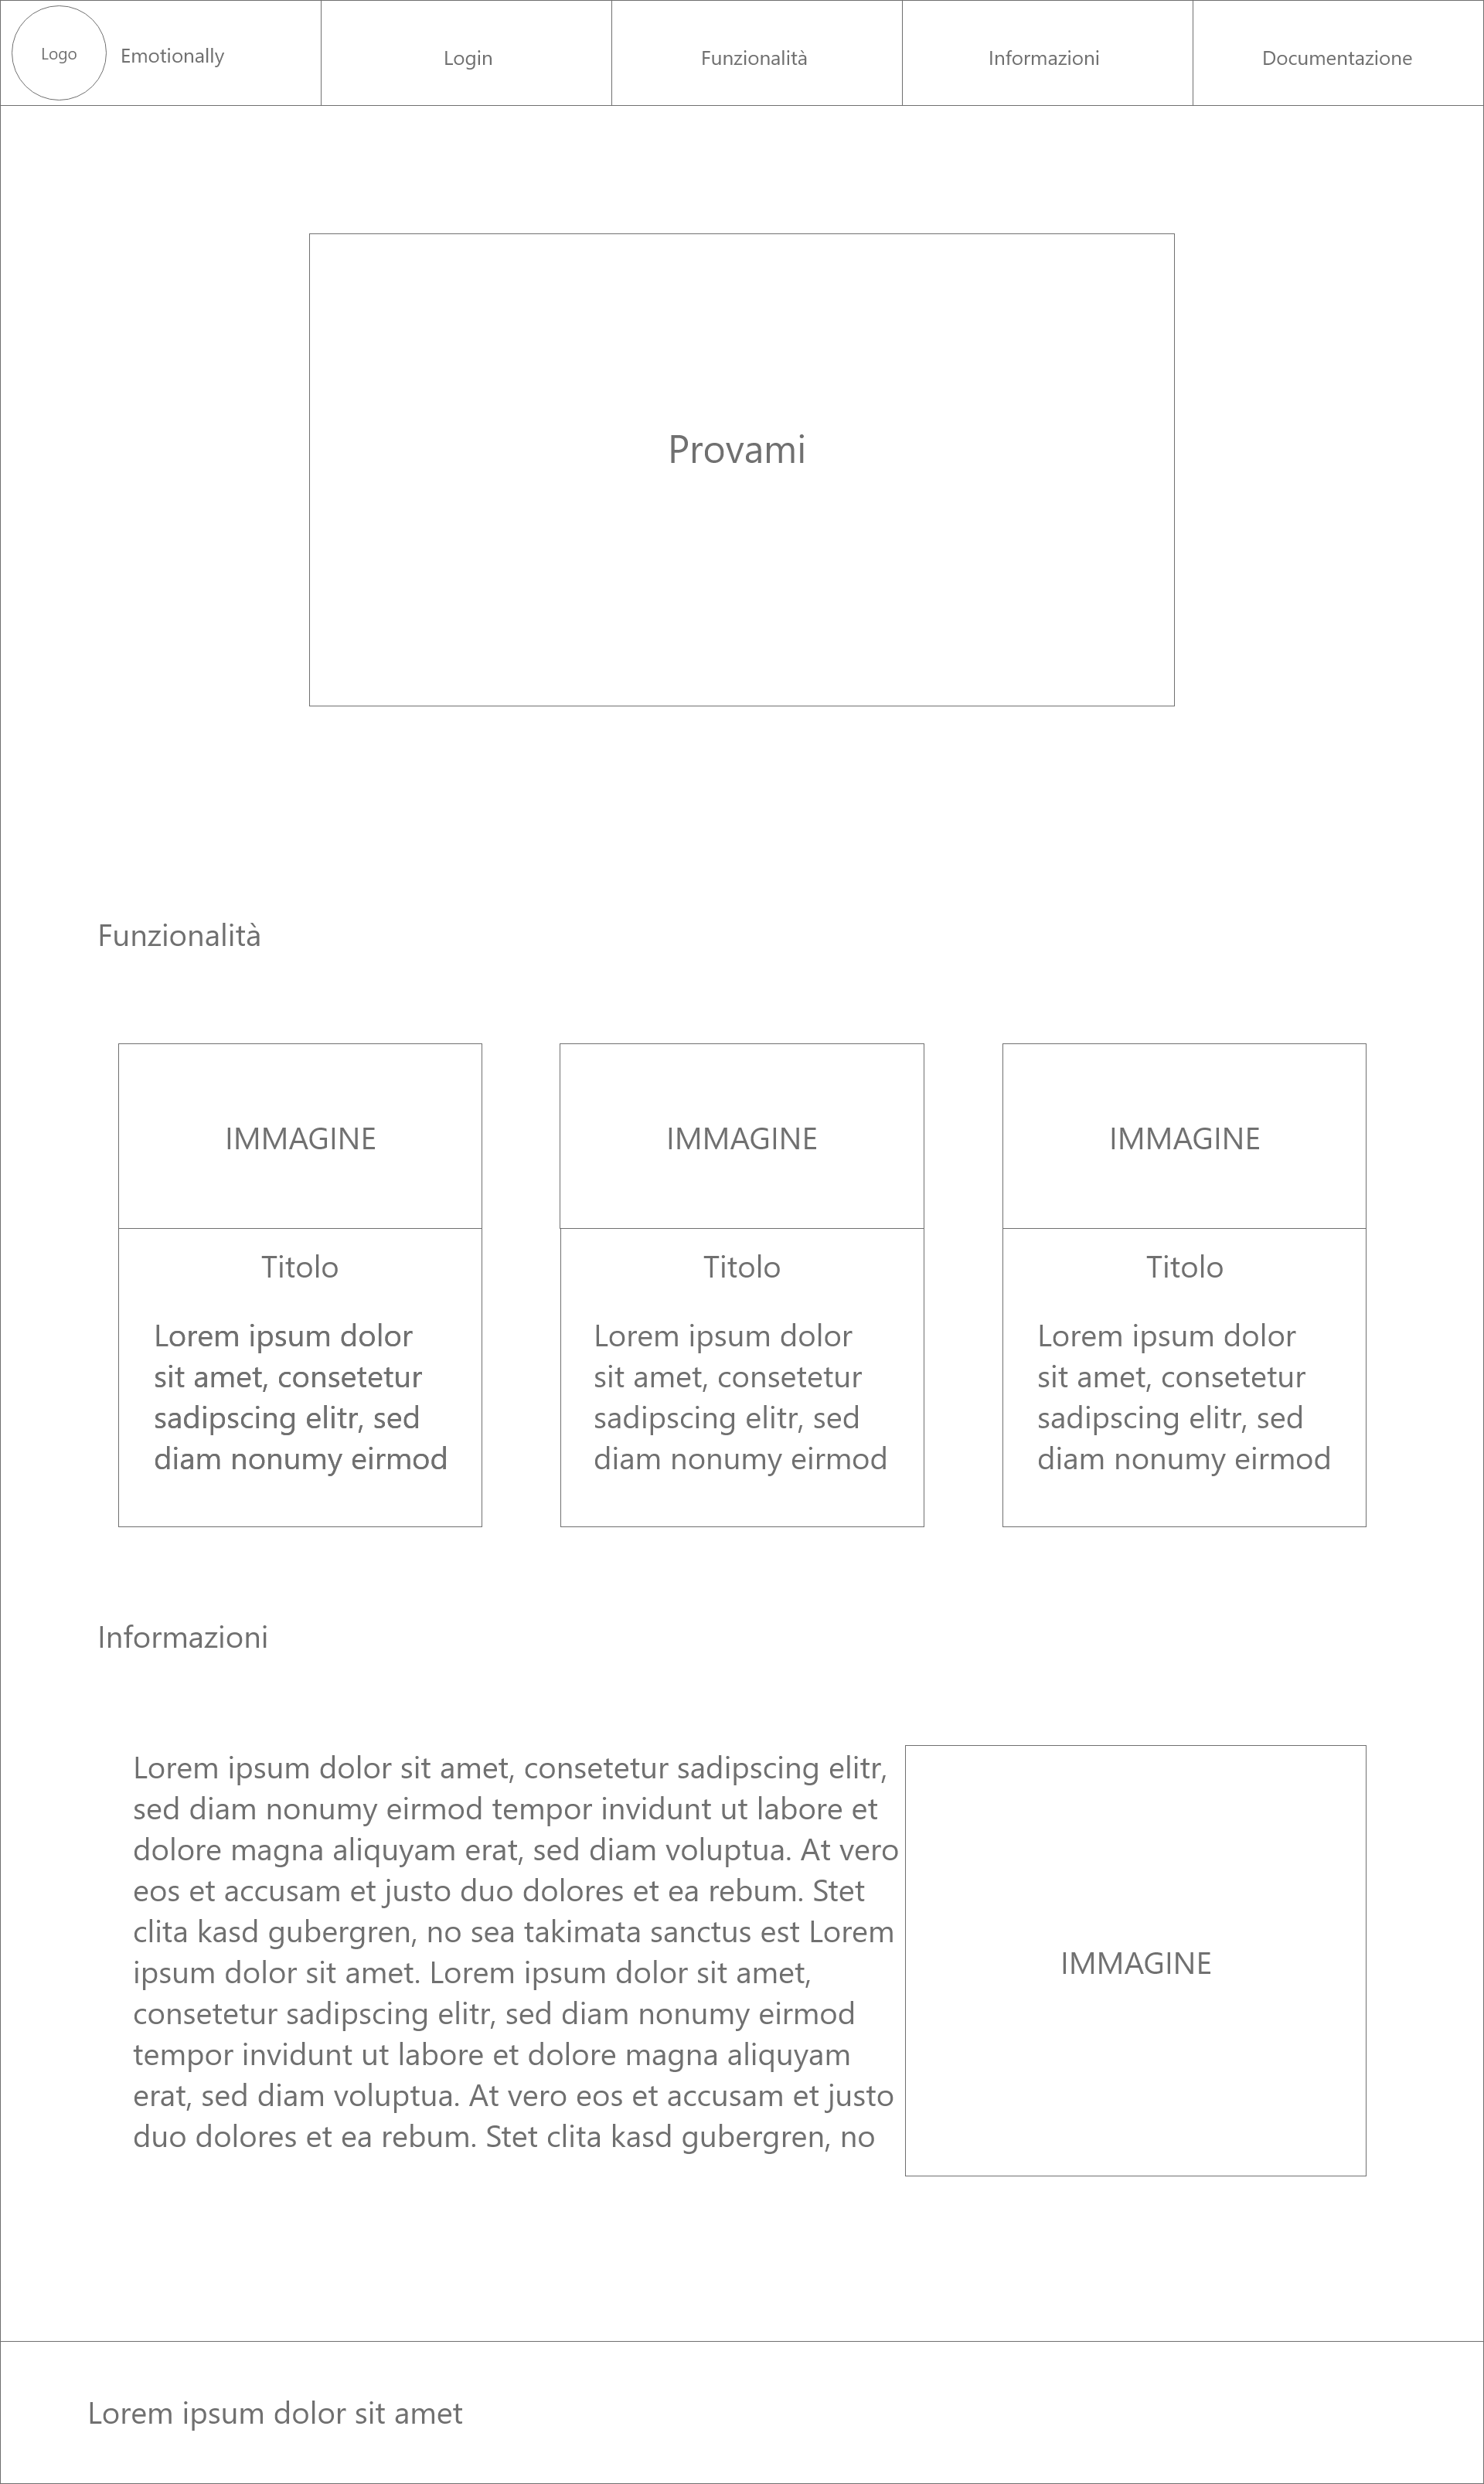
\includegraphics[height=\textheight-3ex]{images/gabbie-logiche/Landing}
\end{figure}

\begin{figure}[H]
	\centering

	\caption{Gabbia logica della pagina di registrazione.}
	\label{fig:gabbie-logiche:registrazione}
	
\includegraphics[width=\textwidth]{images/gabbie-logiche/Registrazione}
\end{figure}

\begin{figure}[H]
	\centering
	\caption{Gabbia logica della home page.}
	\label{fig:gabbie-logiche:home-page}
	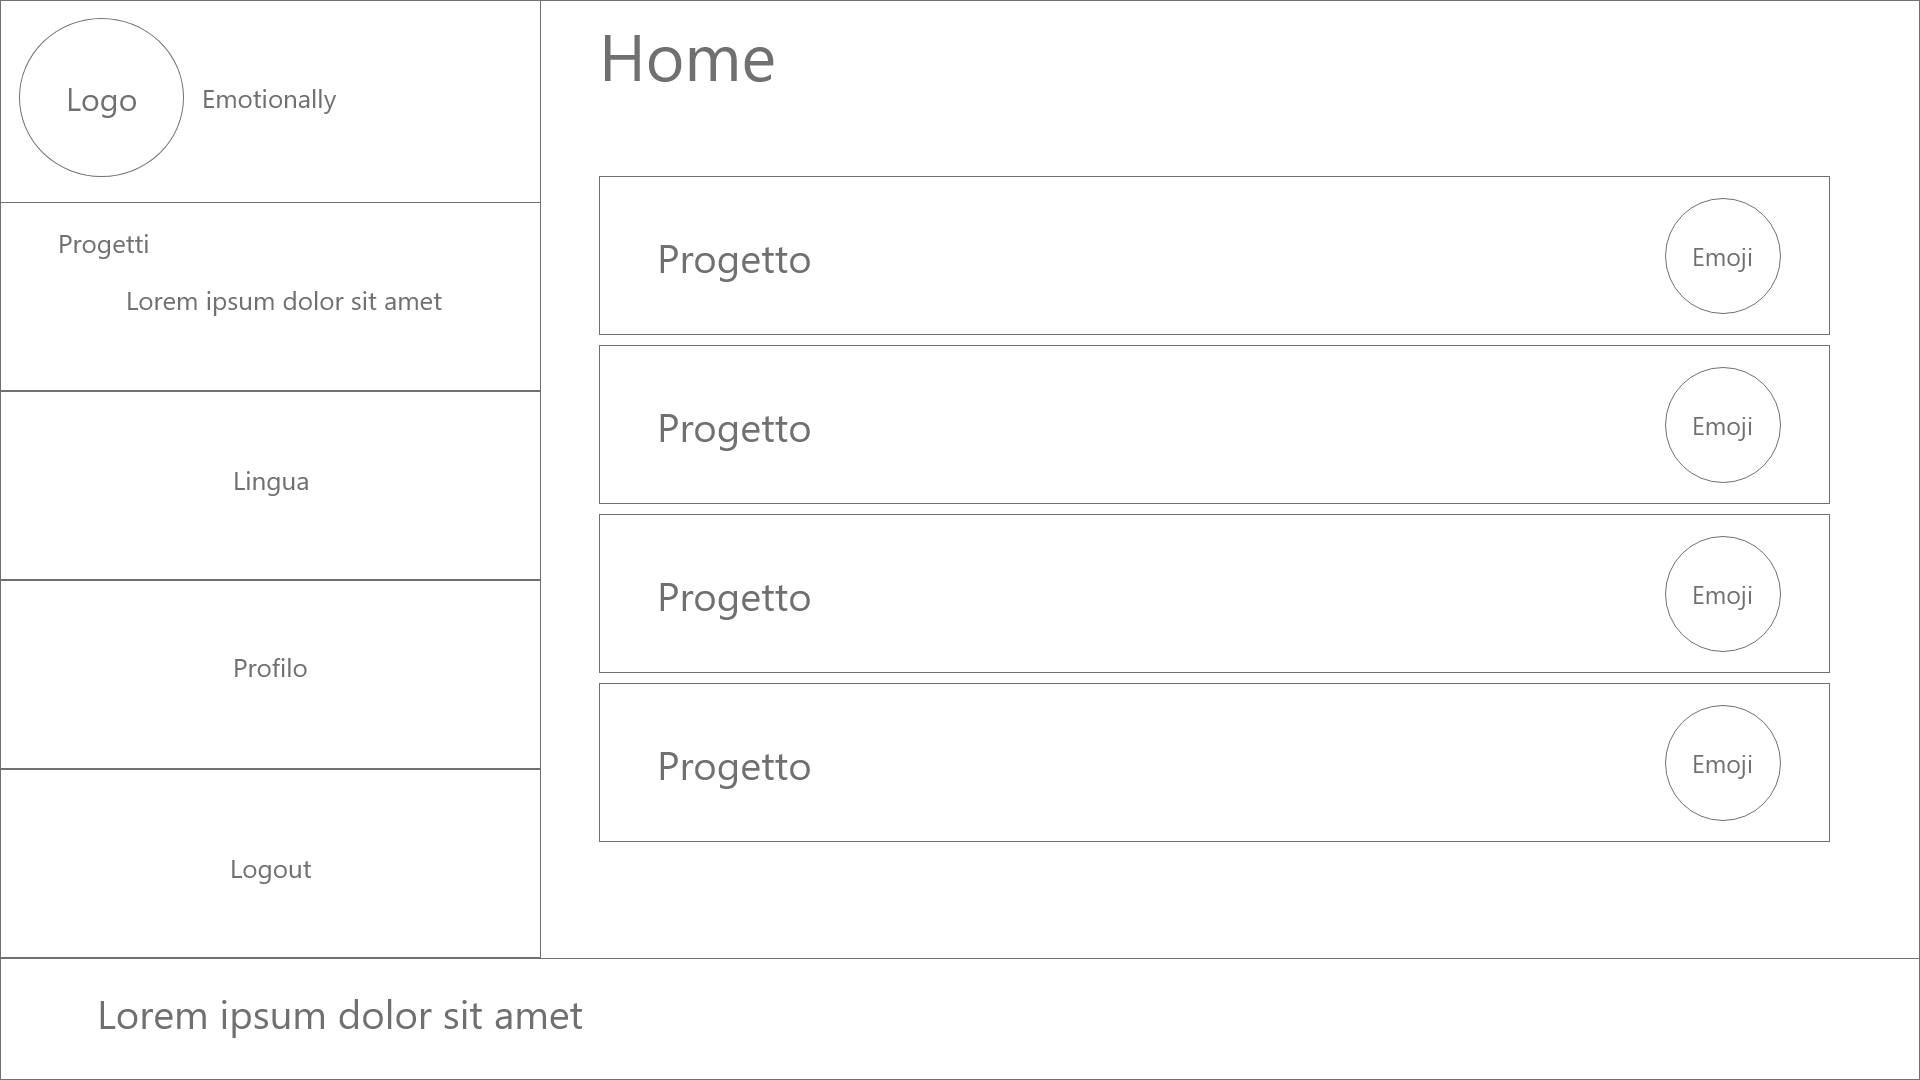
\includegraphics[width=\textwidth]{images/gabbie-logiche/Home}
\end{figure}

\begin{figure}[H]
	\centering
	\caption{Gabbia logica della pagina di un progetto.}
	\label{fig:gabbie-logiche:project}
	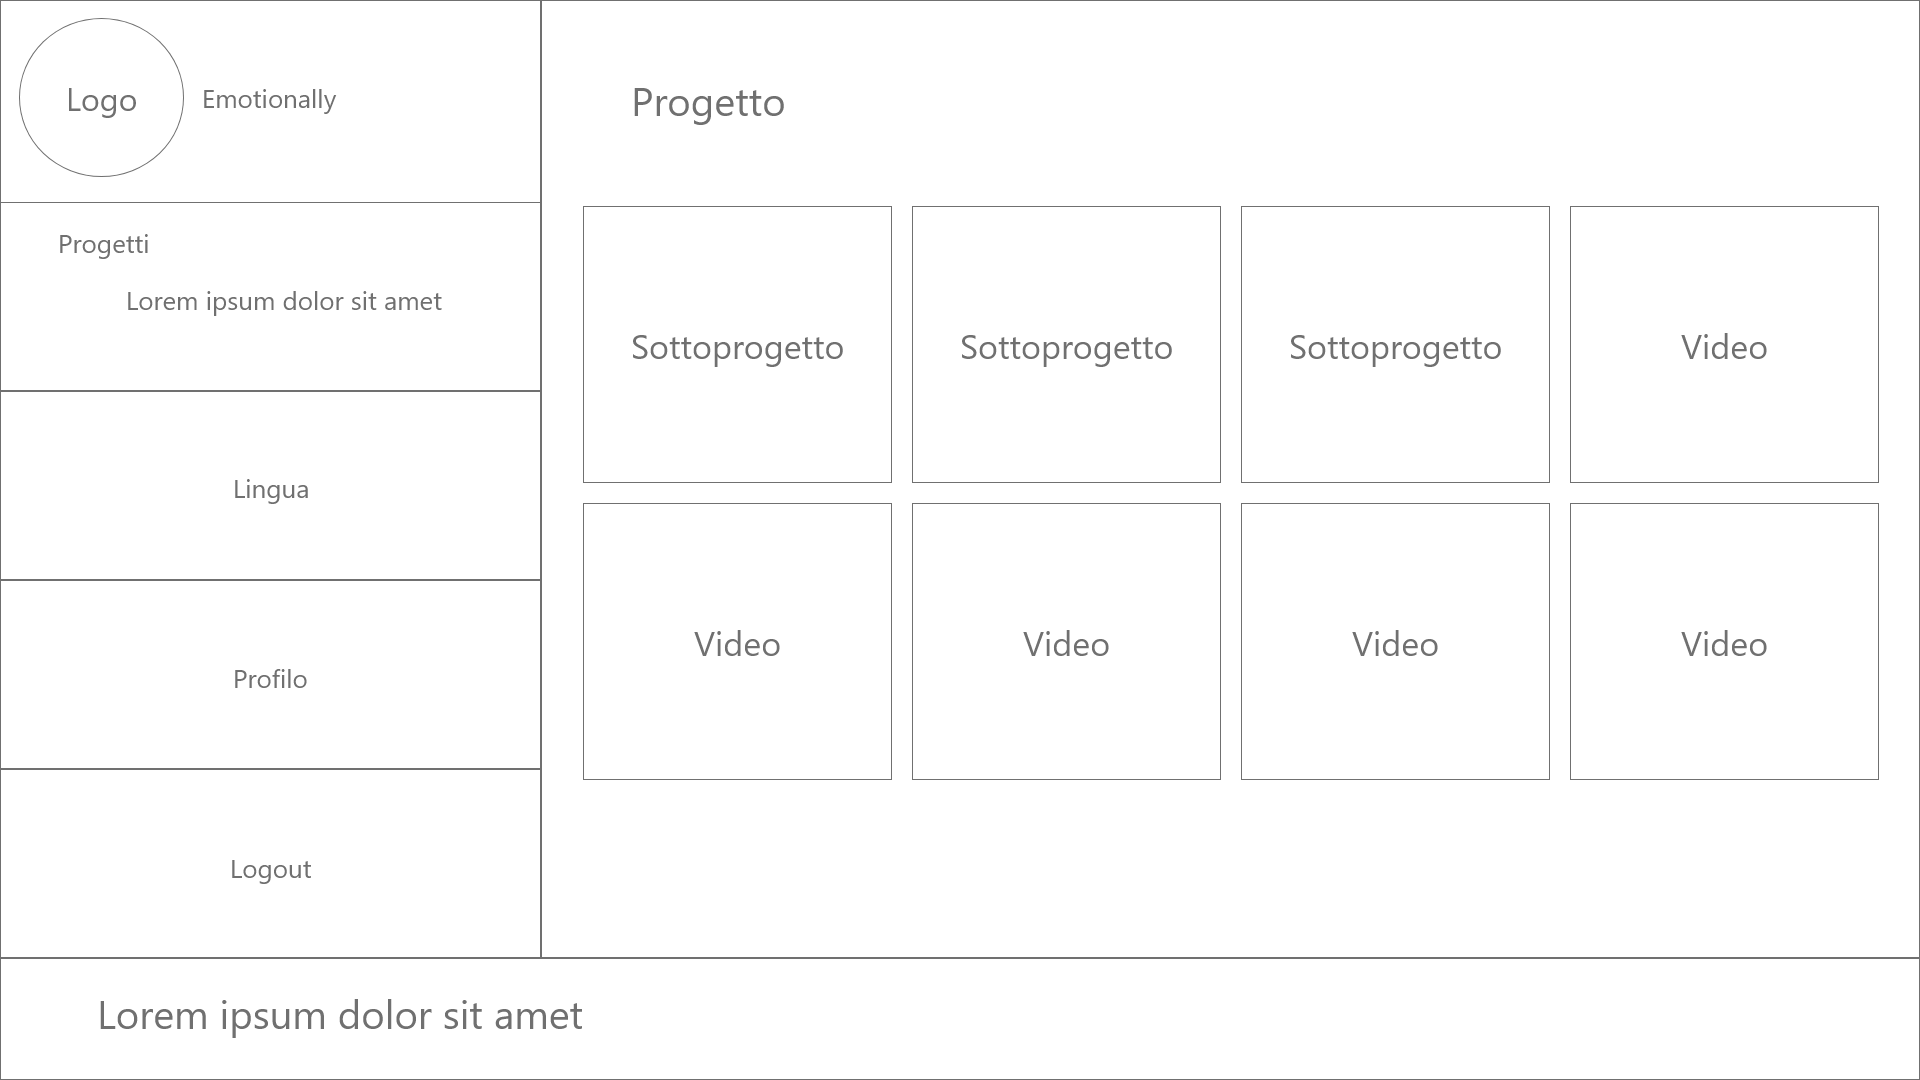
\includegraphics[width=\textwidth]{images/gabbie-logiche/Progetto}
\end{figure}

\begin{figure}[H]
	\centering
	\caption{Gabbia logica della pagina di un video.}
	\label{fig:gabbie-logiche:video}
	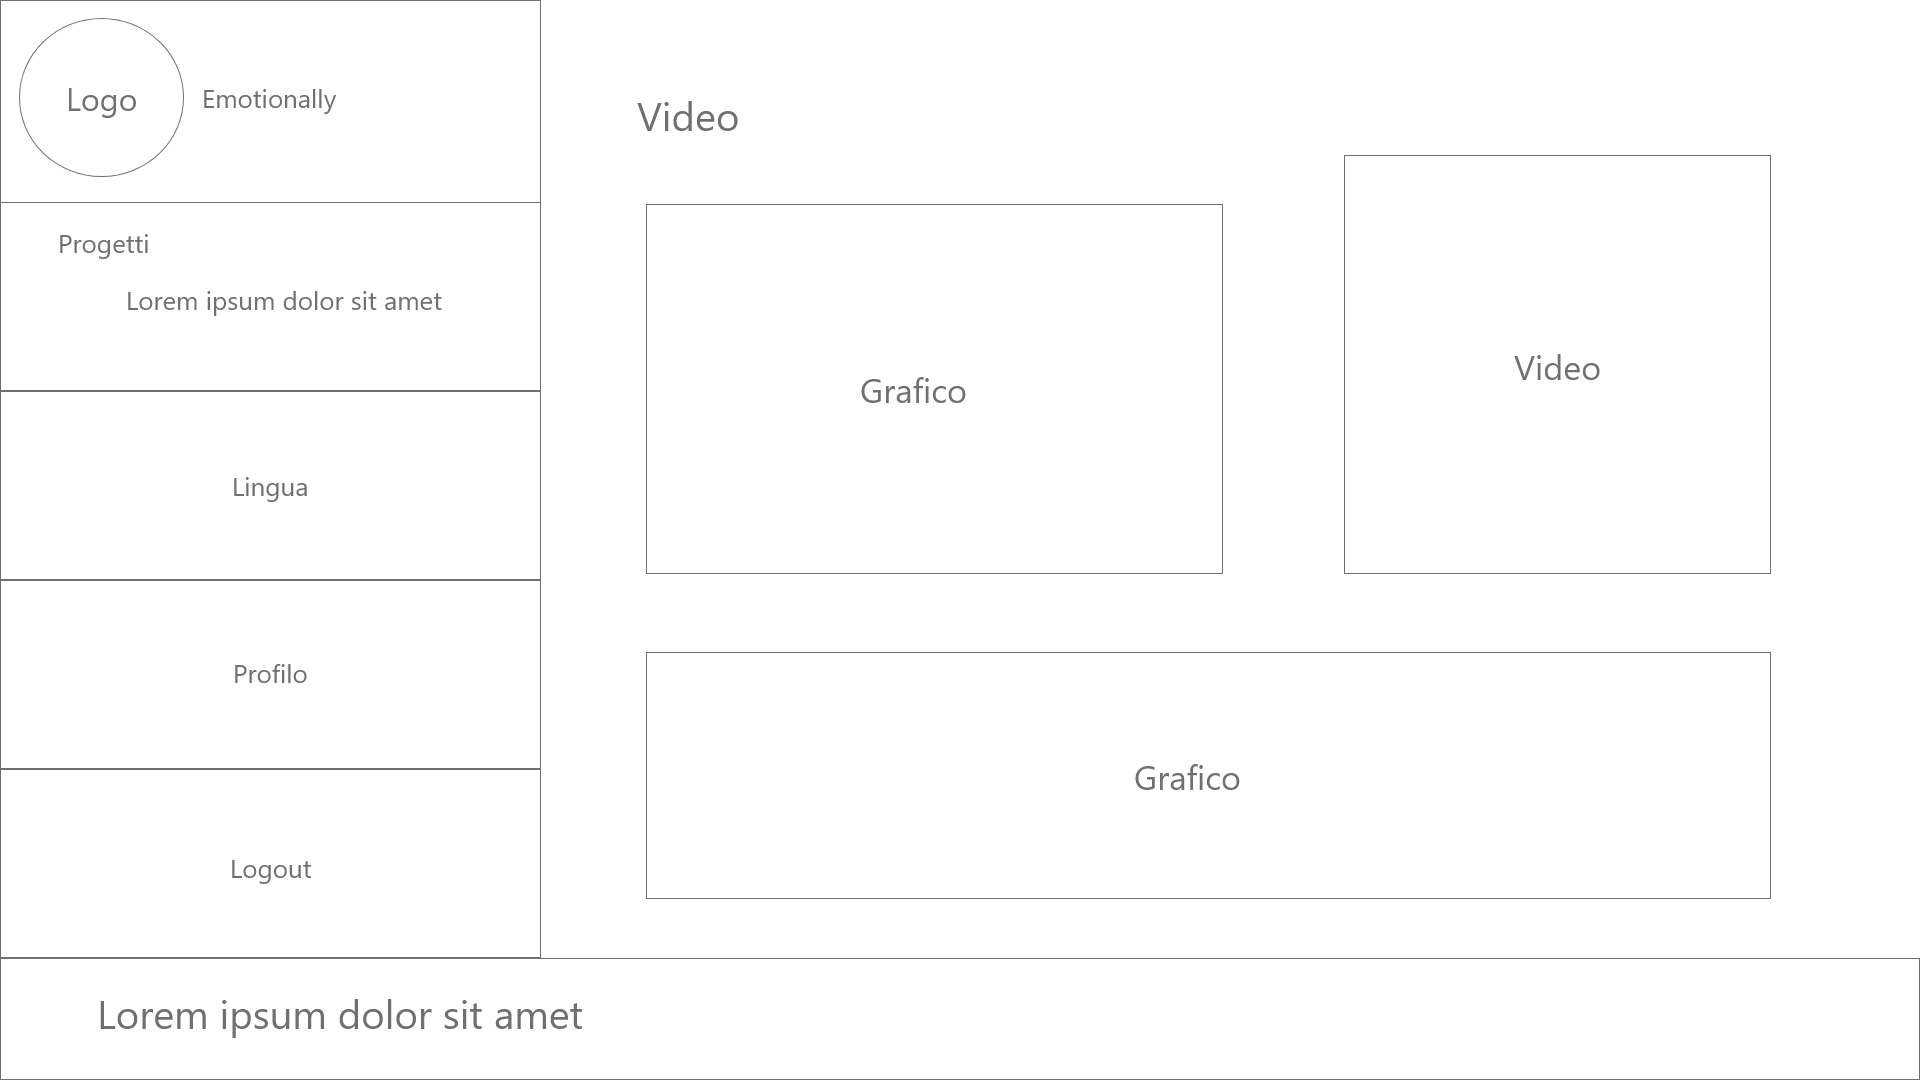
\includegraphics[width=\textwidth]{images/gabbie-logiche/Video}
\end{figure}

\begin{figure}[H]
	\centering
	\caption{Gabbia logica della pagina di profilo.}
	\label{fig:gabbie-logiche:profilo}
	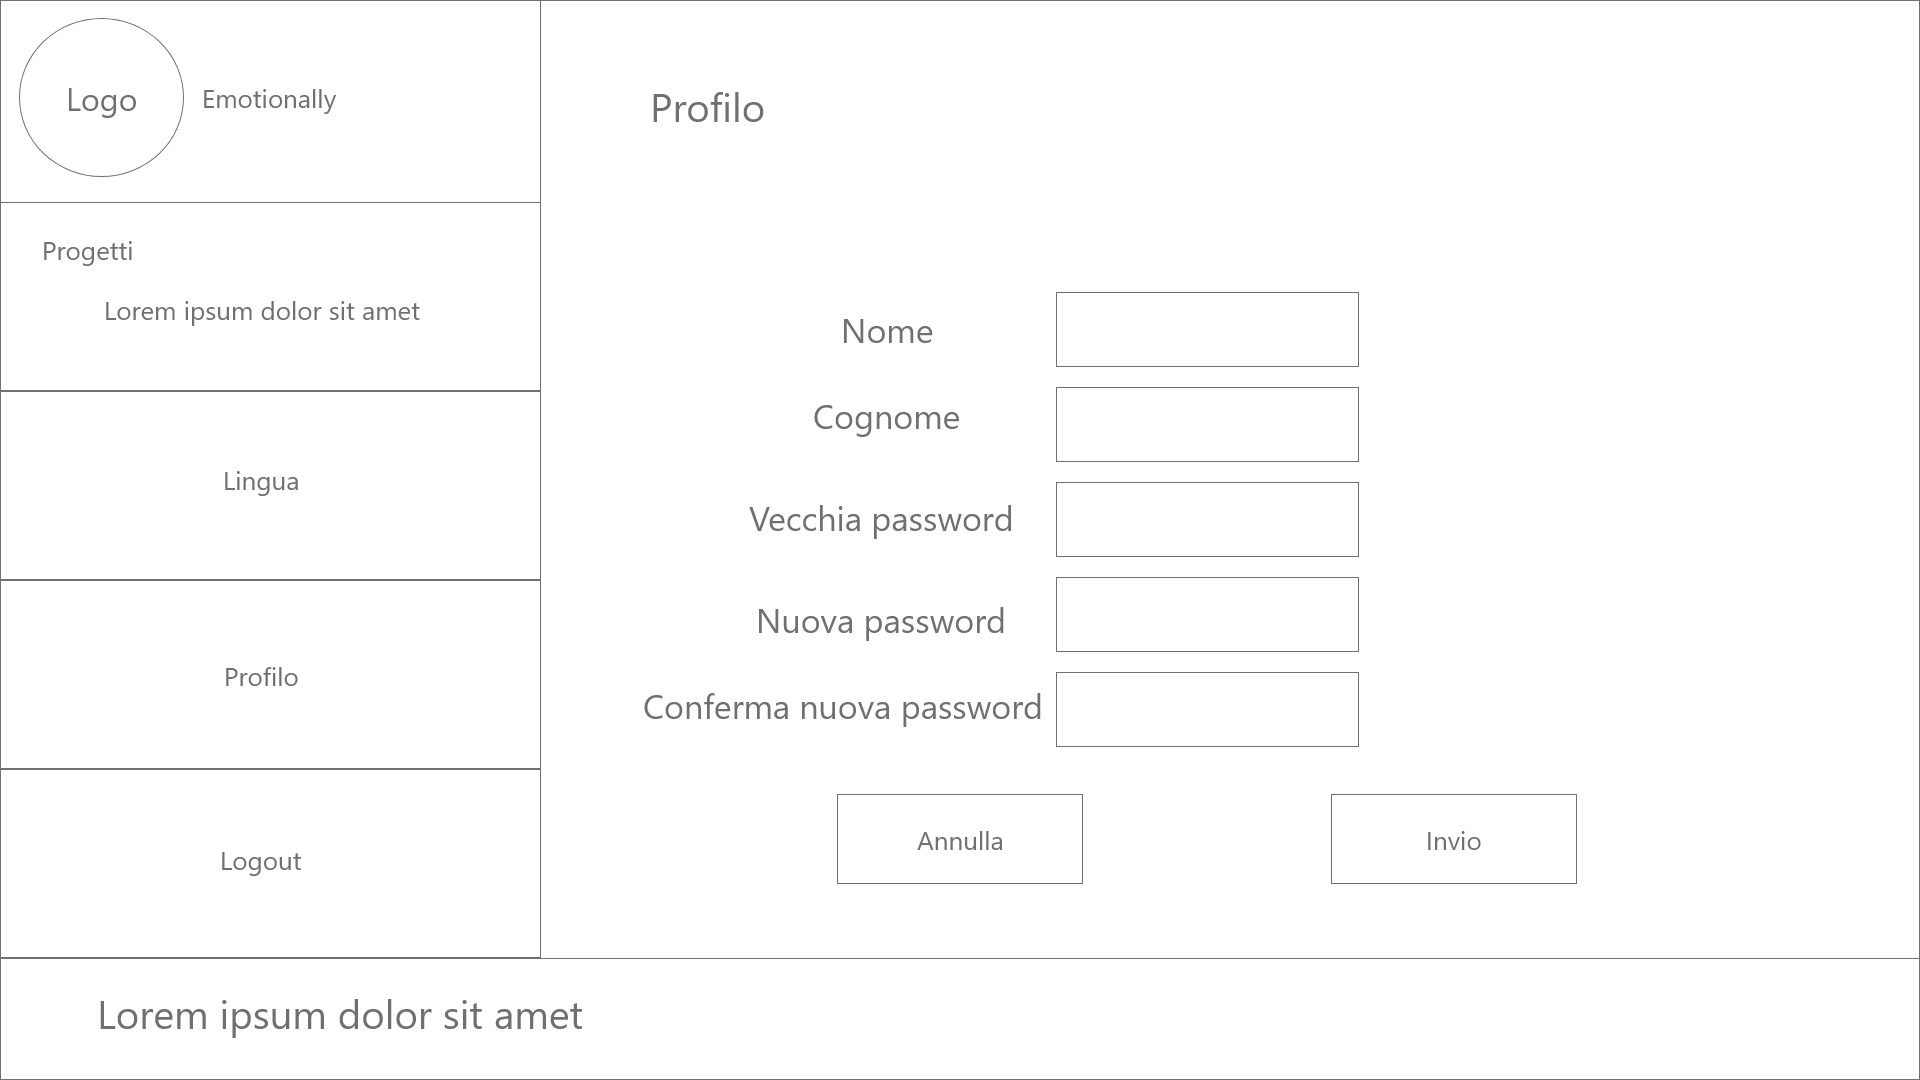
\includegraphics[width=\textwidth]{images/gabbie-logiche/Profilo}
\end{figure}

\begin{figure}[H]
	\centering
	\caption{Gabbia logica della pagina del sottoprogetto.}
	\label{fig:gabbie-logiche:sottoprogetto}
	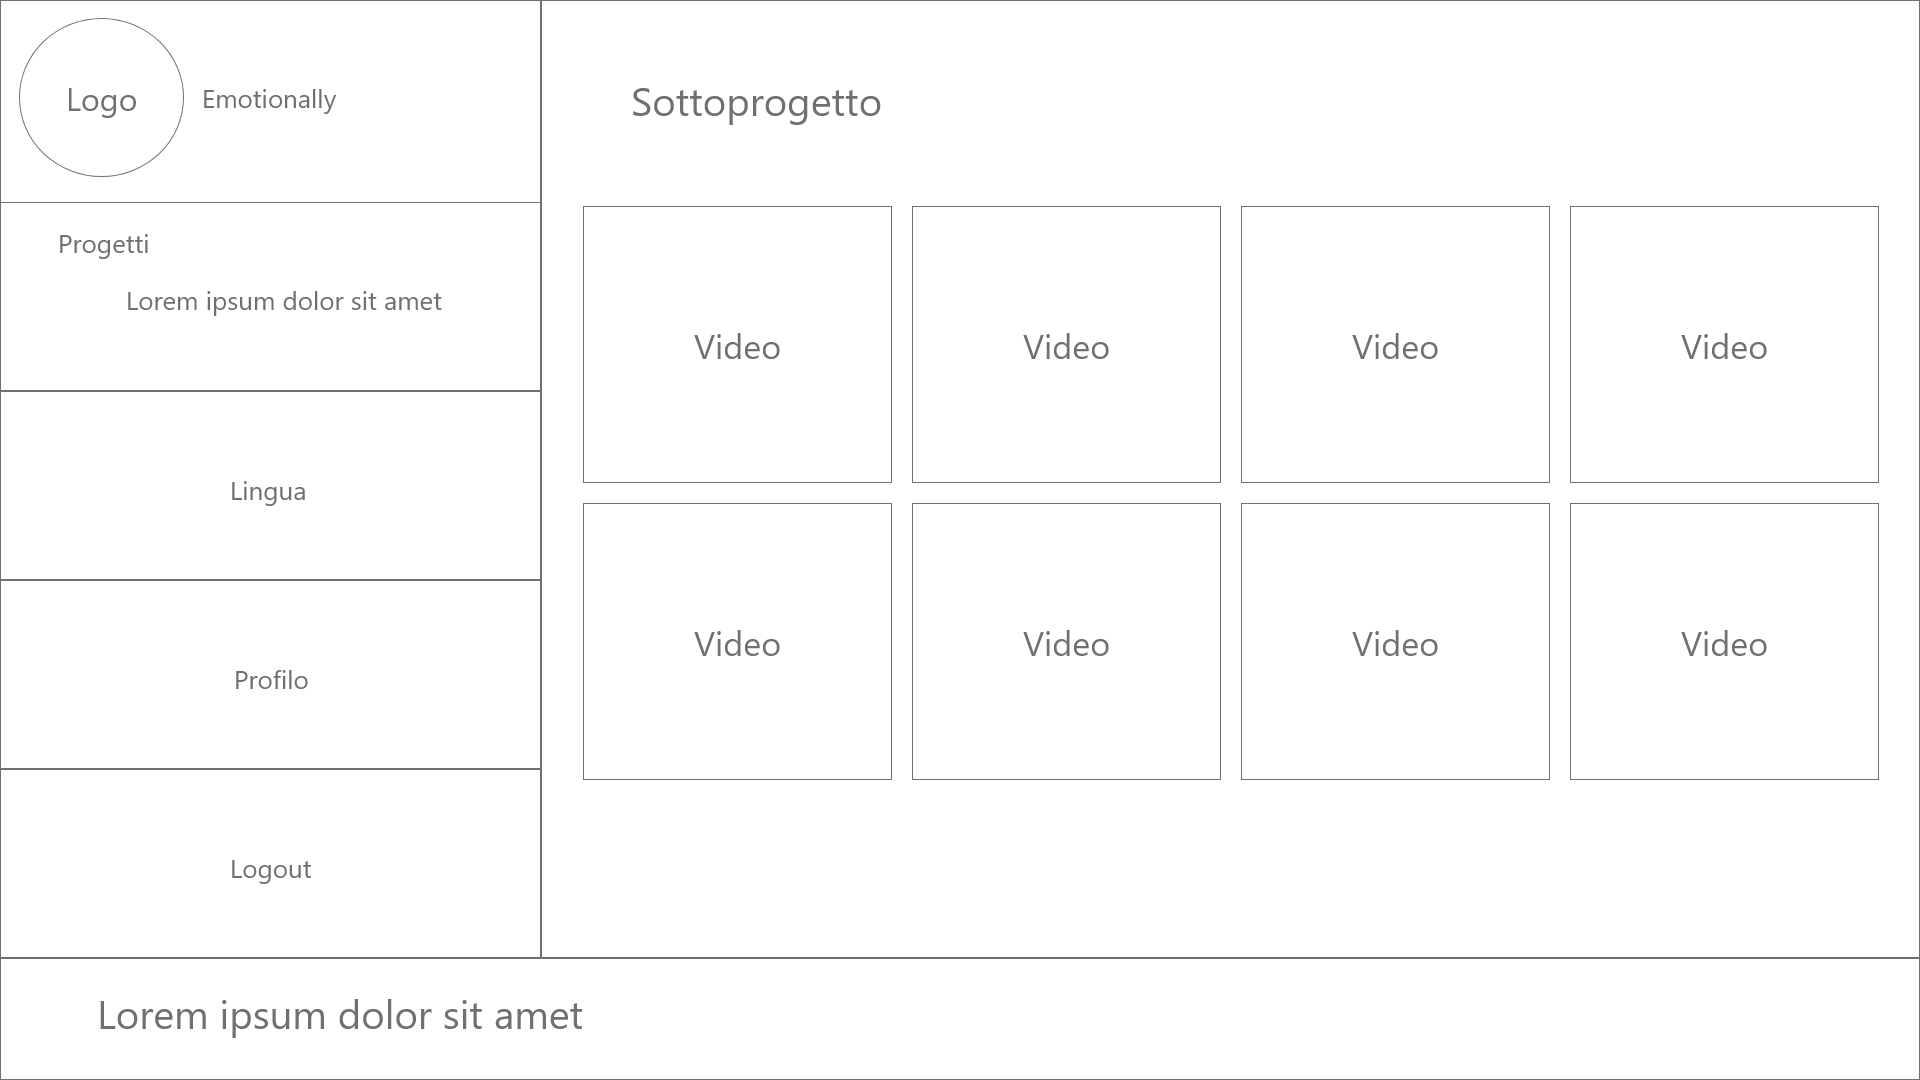
\includegraphics[width=\textwidth]{images/gabbie-logiche/Sottoprogetto}
\end{figure}
